\documentclass[bluish,slideColor,colorBG,pdf]{prosper}
\hypersetup{pdfpagemode=FullScreen}
\usepackage{graphicx}
\def\baselinestretch{1.0}
\setlength{\topmargin}{-60pt}
\setlength{\textheight}{460pt}
\setlength{\oddsidemargin}{0pt}
\setlength{\evensidemargin}{0pt}
\setlength{\textwidth}{660pt}
\setlength{\footskip}{0pt}
\parindent 0.3in
\hyphenpenalty=10000
\tolerance=10000
\pagestyle{empty}

\def\Prob{{\rm Prob\;}}
\def\prob{{\rm \;Prob\;}}


\author{January 2016}
\title{Genome 570, Phylogenetic Inference}
\institution{Week 1:  Parsimony, tree enumeration}

\begin{document}

\maketitle

\begin{slide}[Replace]{A simple data set}
\bigskip

\begin{center}
\renewcommand{\arraystretch}{1.3}
\begin{tabular}{l | l | c c c c c c |}
\cline{3-8}
\multicolumn{2}{c}{}& \multicolumn{6}{|c|}{Characters}\\
\multicolumn{2}{r |}{Species} & 1 & 2 & 3 & 4 & 5 & 6 \\
\cline{2-8}
&Alpha\raisebox{5pt}{\strut} & 1 & 0 & 0 & 1 & 1 & 0\\
&Beta  & 0 & 0 & 1 & 0 & 0 & 0\\
&Gamma & 1 & 1 & 0 & 0 & 0 & 0\\
&Delta & 1 & 1 & 0 & 1 & 1 & 1\\
&Epsilon & 0 & 0 & 1 & 1 & 1 & 0\\
\cline{2-8}
\end{tabular}
\end{center}

\end{slide}

\begin{slide}[Replace]{The tree we will evaluate}

\centerline{\includegraphics[width=4in]{fig1-1.idraw}}

\end{slide}

\begin{slide}[Replace]{Character 1}

\centerline{\includegraphics[width=1.5in]{data1.ydraw} \hspace{0.5in} \includegraphics[width=2in]{fig1-2.idraw}}

\end{slide}

\begin{slide}[Replace]{Character 2}

\centerline{\includegraphics[width=1.5in]{data2.ydraw} \hspace{0.5in} \includegraphics[width=2in]{fig1-3.idraw}}

\end{slide}

\begin{slide}[Replace]{Character 3}

\centerline{\includegraphics[width=1.5in]{data3.ydraw} \hspace{0.5in} \includegraphics[width=2in]{fig1-4.idraw}}

\end{slide}

\begin{slide}[Replace]{Character 4 (and 5)}

\centerline{\includegraphics[width=1.5in]{data4.ydraw} \hspace{0.5in} \includegraphics[width=2in]{fig1-5.idraw}}

\end{slide}

\begin{slide}[Replace]{Character 6}

\centerline{\includegraphics[width=1.5in]{data6.ydraw} \hspace{0.5in} \includegraphics[width=2in]{fig1-6.idraw}}

\end{slide}

\begin{slide}[Replace]{Changes in all characters}
\bigskip

\centerline{\includegraphics[width=4in]{fig1-7.idraw}}

\centerline{There are a total of 9 changes.}

\end{slide}

\begin{slide}[Replace]{Finding a better tree}
\bigskip

\centerline{\includegraphics[width=4in]{fig1-7a.idraw}}

Moving one species, Delta ...

\end{slide}

\begin{slide}[Replace]{Moving it to a new position ... }
\bigskip

\centerline{\includegraphics[width=4in]{fig1-8a.idraw}}

We end up with a tree with 8 changes.

\end{slide}

\begin{slide}[Replace]{Changes on the most parsimonious tree}
\bigskip

\centerline{\includegraphics[width=4in]{fig1-8b.idraw}}

And 8 turns out to be the smallest possible number of changes.

\end{slide}

\begin{slide}[Replace]{Another rooted tree with same number of changes}
\bigskip

\centerline{\includegraphics[width=4in]{fig1-9.idraw}}

\end{slide}

\begin{slide}[Replace]{The corresponding unrooted tree}

\centerline{\includegraphics[width=4in]{fig1-10.idraw}}
\bigskip

The changes placed on the tree really delimit regions of the tree that are
reconstructed to have particular states. 

\end{slide}

\begin{slide}[Replace]{The corresponding unrooted tree}

\centerline{\includegraphics[width=4in]{fig1-10a.idraw}}
\bigskip

If we place the root of the tree
in a different location, the direction of some of the changes is altered, but
not the number of these boundaries of the state regions.
\medskip

(This is true if changes in both directions have the same ``cost'').

\end{slide}

\begin{slide}[Replace]{Using an outgroup to root an unrooted tree}
\bigskip

\centerline{\includegraphics[height=2in]{reroot00.idraw}}
\bigskip

If we have inferred an unrooted tree ...

\end{slide}

\begin{slide}[Replace]{Using an outgroup to root an unrooted tree}
\bigskip

\centerline{\includegraphics[height=2in]{reroot0.idraw}}
\bigskip

... and we know that one branch (here, the branch to Mouse) is the one
where the root connects, then that prior knowledge roots the tree.  That
group or species is the ``outgroup''.  This amounts to the prior knowledge
that the rest of the tree is a monophyletic group (the ``ingroup'').

\end{slide}

\begin{slide}[Replace]{Using an outgroup to root an unrooted tree}
\bigskip

\centerline{\includegraphics[height=2in]{reroot1.ydraw}}
\bigskip

If instead we have this unrooted tree, and we add to the data set the
species Mouse, which will be our outgroup ...

\end{slide}

\begin{slide}[Replace]{Using an outgroup to root an unrooted tree}
\bigskip

\centerline{\includegraphics[height=2in]{reroot2.ydraw}}
\bigskip

... it adds information by attaching to one branch or another.
Then we use our prior assumption that the root is on the branch
between Mouse and whatever node to which it attaches.

\end{slide}

\begin{slide}[Replace]{Branch lengths, averaging over reconstructions}
\vspace{0.4in}

\centerline{\includegraphics[width=4in]{fig1-11.idraw}}

\end{slide}

\begin{slide}[Replace]{Walter Fitch (1929-2011) }
\vspace{0.2in}

\centerline{\includegraphics[width=1.2in]{Fitch3a.ps}}
\bigskip

\centerline{Walter Fitch, in 1975}

\end{slide}

\begin{slide}[Replace]{The Fitch algorithm}

To count steps at a site:

\begin{enumerate}
\setlength{\itemsep}{4pt}
\item At the tips of the tree, make a set with those nucleotides which
are possible at that tip (more than one if there is ambiguity)
\item Go down the tree (perhaps by postorder tree traversal), considering
each node only after its two descendants have been considered.
\item At each interior node, construct the set as the intersection of
the two descendant sets:
\[
\mathsf{S_n \  = \  S_\ell \ \cap \ S_r}
\]
\item If this is empty, instead construct the union of the two
descendant sets, and count one step:
\[
\mathsf{S_n \  = \  S_\ell \ \cup \ S_r}
\]
\item Continue to the bottom node.  The count of steps is the total
of these counts.
\end{enumerate}

\end{slide}

\begin{slide}[Replace]{Example for the Fitch algorithm}

\centerline{\includegraphics[width=4in]{fig2-1a.ydraw}}

\end{slide}

\begin{slide}[Replace]{Example for the Fitch algorithm}

\centerline{\includegraphics[width=4in]{fig2-1b.ydraw}}

\end{slide}

\begin{slide}[Replace]{Example for the Fitch algorithm}

\centerline{\includegraphics[width=4in]{fig2-1c.ydraw}}

\end{slide}

\begin{slide}[Replace]{Example for the Fitch algorithm}

\centerline{\includegraphics[width=4in]{fig2-1d.ydraw}}

\end{slide}

\begin{slide}[Replace]{Example for the Fitch algorithm}

\centerline{\includegraphics[width=4in]{fig2-1e.ydraw}}

\end{slide}

\begin{slide}[Replace]{Shortest path through a graph}

\centerline{\includegraphics[height=3in]{graphpath1.idraw}}

\end{slide}

\begin{slide}[Replace]{Shortest path through a graph}

\centerline{\includegraphics[height=3in]{graphpath3.idraw}}

\end{slide}

\begin{slide}[Replace]{Shortest path through a graph}

\centerline{\includegraphics[height=3in]{graphpath5.idraw}}

\end{slide}

\begin{slide}[Replace]{Shortest path through a graph}

\centerline{\includegraphics[height=3in]{graphpath6.idraw}}

\end{slide}

\begin{slide}[Replace]{Shortest path through a graph}

\centerline{\includegraphics[height=3in]{graphpath7.idraw}}

\end{slide}

\begin{slide}[Replace]{Shortest path through a graph}

\centerline{\includegraphics[height=3in]{graphpath8.idraw}}

\end{slide}

\begin{slide}[Replace]{We finally get scores for all nodes}

\centerline{\includegraphics[height=3in]{graphpath97.idraw}}

\end{slide}

\begin{slide}[Replace]{Then we go back from goal}

\centerline{\includegraphics[height=3in]{graphpath98.idraw}}

\end{slide}

\begin{slide}[Replace]{This is a `dynamic programming' algorithm}

\centerline{\includegraphics[height=3in]{graphpath99.idraw}}

\end{slide}

\begin{slide}[Replace]{Parsimony is a shortest-path problem}

\centerline{\includegraphics[height=3in]{prunepaths.idraw}}

\end{slide}

\begin{slide}[Replace]{David Sankoff}

\centerline{\includegraphics[width=2in]{sankoff4.ps}}
\bigskip

\centerline{David Sankoff, in the 1990s, writing on a glass panel}
\centerline{(forwards, then he went behind it)}

\end{slide}

\begin{slide}[Replace]{The Sankoff algorithm}

\begin{center}
\begin{tabular}{c c c}
\includegraphics[height=1in]{sankoffalr.idraw} &
\hspace{0.5in} &
\includegraphics[height=1in]{compflow.idraw}
\end{tabular}
\end{center}

\begin{enumerate}
\setlength{\itemsep}{4pt}
\item $\mathsf{S_k(i)~}$ is defined as the number of steps required at or above
node $\mathsf{~k~}$ given that node $\mathsf{~k~}$ is in state $\mathsf{~i}$.
\item Set these quantities at the tips for the character (they are either 0 or $\infty$).
\item move down the tree doing this at each node:
\[
\mathsf{S_a(i) \  = \  \min_j \left[ c_{ij} + S_\ell(j)\right] \ + \  \min_k
\left[ c_{ik}
+ S_r(k)\right]}
\]
\item At the bottom node of the tree:
\[
\mathsf{S \ = \ \min_i S_0(i)}
\]
\end{enumerate}

\end{slide}

\begin{slide}[Replace]{Example for the Sankoff algorithm}

\centerline{\includegraphics[width=4.4in]{fig2-2.idraw}}

\end{slide}

\begin{slide}[Replace]{Economizing on the score computation}

\centerline{\includegraphics[width=2.2in]{fig2-3.idraw}}
\bigskip

By retaining the interior arrays of scores, we can avoid having to
redo the parts of the tree that have not changed.  The result is a
great speedup if only a small part of the tree has changed.

\end{slide}

\begin{slide}[Replace]{The same tree? }

\centerline{\includegraphics[width=3.8in]{fig3-1.idraw}}
\bigskip

(It's important that you know how to answer this.  Also that you be able
to recognize whether two different rooted trees are the same unrooted tree).

\end{slide}

\begin{slide}[Replace]{Rooted, labelled, bifurcating trees}

\centerline{\includegraphics[width=2in]{fig3-2.idraw}}

\end{slide}

\begin{slide}[Replace]{Adding species in all possible places}

\centerline{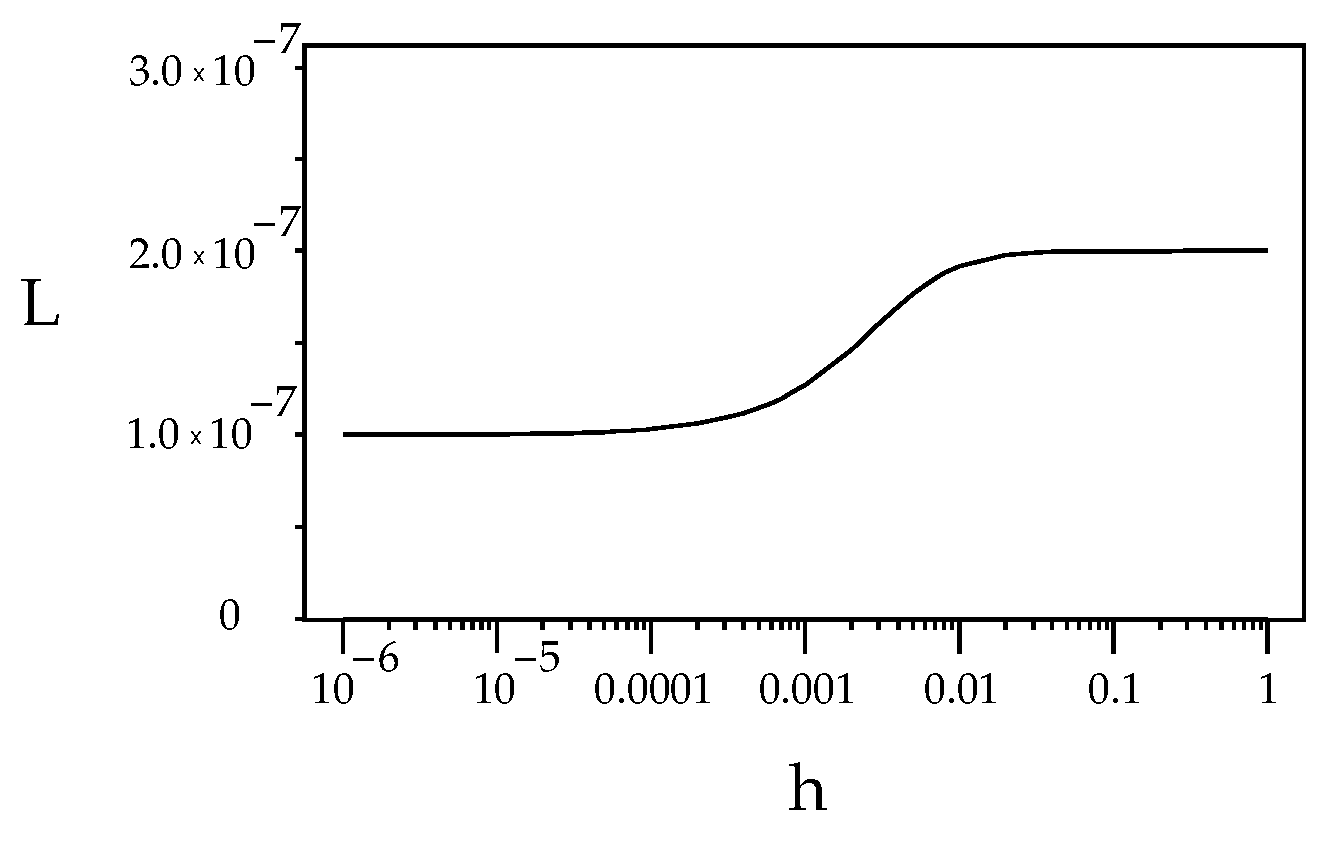
\includegraphics[width=2.2in]{fig3-3.idraw}}

\end{slide}

\begin{slide}[Replace]{The resulting count of the number of trees}
\bigskip

{\large
\[
\mathsf{1 \times 3 \times 5 \times 7 \times 9 \times \dots \times (2n-3)} 
\]
}
\bigskip

We can get this from the argument about adding species in a particular
order (say, alphabetically) in all possible places on the tree.  Once we
realize that all rooted bifurcating trees with that set of species can be
reached this way, and that each one can be reached in only one such way,
it becomes obvious that the above product counts the number of possible trees.

\end{slide}

\begin{slide}[Replace]{Rooted, bifurcating, labelled trees}

\vspace{-0.1in}

{\ptsize{8}
\begin{center}
\renewcommand{\arraystretch}{0.85}
\begin{tabular}{r r}
species & number of trees \\
\hline
1 & 1 \\
2 & 1 \\
3 & 3 \\
4 & 15 \\
5 & 105 \\
6 & 945 \\
7 & 10,395 \\
8 & 135,135 \\
9 & 2,027,025 \\
10 & 34,459,425 \\
11 & 654,729,075\\
12 & 13,749,310,575\\
13 & 316,234,143,225\\
14 & 7,905,853,580,625\\
15 & 213,458,046,676,875\\
16 & 6,190,283,353,629,375\\
17 & 191,898,783,962,510,625\\
18 & 6,332,659,870,762,850,625\\
19 & 221,643,095,476,699,771,875\\
20 & \ \ \ \ \ \ \ \ \ \ 8,200,794,532,637,891,559,375\\
30 & 4.9518 $\times 10^{38}$\\
40 & 1.00985 $\times {\rm 10}^{57}$\\
50 & 2.75292 $\times {\rm 10}^{76}$\\
\end{tabular}
\end{center}
}

\end{slide}

\begin{slide}[Replace]{Rooting an unrooted tree at species 1}

\centerline{\includegraphics[width=4in]{fig3-4.idraw}}
\bigskip

So an unrooted tree can be considered as being a rooted
tree, provided one of the tip species becomes the ``root'' so
that the rooted tree has one fewer species.
\bigskip

Thus the number of unrooted trees is the same as the number of rooted
trees, ones that have one fewer species.

\end{slide}

\begin{slide}[Replace]{Multifurcating trees}

\centerline{\includegraphics[width=3.8in]{fig3-5.idraw}}
\bigskip

Note that they have different numbers of branches as well.  To count them
we have to keep track of the numbers of trees with different numbers of
interior nodes.  Then it is fairly easy.  I introduced this method in 1978;
the number of rooted multifurcating trees was first counted 108 years earlier 
by Ernst Schr\"oder in 1870 using generating function methods.

\end{slide}

\begin{slide}[Replace]{Counting multifurcating rooted trees}
\bigskip

If we add a new species to a tree that has $\mathsf{~n~}$ tips and
$\mathsf{~m~}$ interior nodes, there are two kinds of places we could add them:

\begin{enumerate}
\item Branching off of one of the $\mathsf{~n+m~}$ branches.
\item Coming out of one of the $\mathsf{~m~}$ interior nodes.
\end{enumerate}

Each of these generates a different new tree.  Branching off of a branch
creates a new interior node, coming out of an interior node does not create a
new interior node.

\end{slide}

\begin{slide}[Replace]{The algorithm counting multifurcating rooted trees}

\centerline{\includegraphics[width=3.2in]{fig3-6.idraw}}

\end{slide}

\begin{slide}[Replace]{Rooted trees allowing multifurcations}

\vspace{-0.1in}
{\ptsize{8}
\begin{center}
\renewcommand{\arraystretch}{0.85}
\begin{tabular}{r r}
 {\rm species} & {\rm number of trees}\\
\hline
 2 & 1\\
 3 & 4\\
 4 & 26\\
 5 & 236\\
 6 & 2,752\\
 7 & 39,208\\
 8 & 660,032\\
 9 & 12,818,912\\
 10 & 282,137,824\\
 11 & 6,939,897,856\\
 12 & 188,666,182,784\\
 13 & 5,617,349,020,544\\
 14 & 181,790,703,209,728\\
 15 & 6,353,726,042,486,272\\
 16 & 238,513,970,965,257,728\\
 17 & 9,571,020,586,419,012,608\\
 18 & 408,837,905,660,444,010,496\\
 19 & 18,522,305,410,364,986,906,624\\
 20 & \ \ \ \ \ \ \ \ \ \ 887,094,711,304,119,347,388,416\\
 30 & 7.0717$ \times 10^{41}$\\
 40 & 1.9037$\times 10^{61}$\\
 50 &   6.85$ \times 10^{81}$\\
 100 &  3.3388$ \times 10^{195}$
\end{tabular}
\end{center}
}

\end{slide}

\begin{slide}[Replace]{Wedderburn's algorithm for numbers of tree shapes}
\bigskip

\[
\begin{array}{c c l l}
\mathsf{S_1} & \mathsf{=} & \mathsf{1} & \\
& & & \\
\mathsf{S_n} & \mathsf{=} & \mathsf{S_1 S_{n-1} + S_2 S_{n-2} + \dots + S_{(n-1)/2} S_{(n+1)/2}} & \mathsf{\mbox{if $n > 1$ and $n$ is odd}}\\
& & & \\
\mathsf{S_n} & \mathsf{=} & \mathsf{S_1 S_{n-1} + S_2 S_{n-2} + \dots + S_{n/2}(\,S_{n/2}+1)/2} & \mathsf{\mbox{if $n > 1$ and $n$ is even}}\\
\end{array}
\]

This algorithm is easily obtained by considering that a rooted bifurcating
tree with $n$ tips has a fork at its base with a tree of $k$ tips on one
side, and a tree of $n-k$ tips on the other, and that exchanging the
order of these does not change the tree.

\end{slide}

\begin{slide}[Replace]{Shapes of rooted bifurcating trees}

\vspace{-0.1in}
{\ptsize{8}
\begin{center}
\renewcommand{\arraystretch}{0.8}
\begin{tabular}{ c r }
\mbox{species}&\mbox{\ \ \ \ \ number of shapes} \\
\hline
1 & 1 \\
2 & 1 \\
3 & 1 \\
4 & 2 \\
5 & 3 \\
6 & 6 \\
7 & 11 \\
8 & 23 \\
9 & 46  \\
10 & 98  \\
11 & 207  \\
12 & 451  \\
13 & 983  \\
14 & 2,179  \\
15 & 4,850  \\
16 & 10,905  \\
17 & 24,631  \\
18 & 56,011  \\
19 & 127,912  \\
20 & 293,547 \\
30 & 1.4068$\times 10^9$\\
40 & 8.0997$\times 10^{12}$\\
50 & 5.1501$\times 10^{16}$\\
100 & \ \ \ \ \ \ \ \ \ \ 1.0196$\times 10^{36}$
\end{tabular}
\end{center}
}

\end{slide}

\begin{slide}[Replace]{Rooted, bifurcating tree shapes}

\centerline{\includegraphics[width=2in]{fig3-7.idraw}}

\end{slide}

\begin{slide}[Replace]{Unrooted bifurcating tree shapes}

\centerline{\includegraphics[width=2.8in]{fig3-8.idraw}}

\end{slide}

\begin{slide}[Replace]{Unrooted multifurcating tree shapes}

\centerline{\includegraphics[width=2.4in]{fig3-9.idraw}}

\end{slide}

\begin{slide}[Replace]{Same topology but different labelled histories}
\bigskip

\centerline{\includegraphics[width=4in]{fig3-10.idraw}}

\end{slide}

\begin{slide}[Replace]{Counting labelled histories}
\bigskip

You can count labelled histories by going back in time, noting that there are
${n \choose 2} \ = \ n(n-1)/2$
different pairs that can join most recently.  Before that there are $n-1$
lineages so there are $(n-1)(n-2)/2$ pairs that can join.  Going all the
way back to the root, just before it $2\times 1/2$ pairs can join. 
\bigskip

Each combination of choices leads to a different labelled history, so we
take the product of these numbers.
\bigskip

This leaves us with
\[
\frac{n! (n-1)!}{2^{n-1}}
\]
labelled histories.

\end{slide}

\begin{slide}[Replace]{The number of labelled histories}
\vspace{-0.27in}

\begin{center}
\[
\begin{array}{ c c r}
  n   &  &   {\rm Number} \\
\hline
  2  &  \ \ \ \ &      1 \\
3  &  &  3 \\
4  &  &  18 \\
5  &  &  180 \\
6  &  &  2700 \\
7  &  &  56700 \\
8  &  &  1587600 \\
9  &  &  57153600 \\
10  & &  2571912000 \\
11  & &  141455160000 \\
12  & &  9.336041\times 10^{12} \\
13  & &  7.282112\times 10^{14} \\
14  & &  6.626722\times 10^{16} \\
15  & &  6.958058\times 10^{18} \\
16  & &  8.349669\times 10^{20} \\
17  & &  1.135555\times 10^{23} \\
18  & &  1.737399\times 10^{25} \\
19  & &  2.970953\times 10^{27} \\
20  & &  5.644810\times 10^{29} \\
\end{array}
\]
\end{center}

\end{slide}

\end{document}

